\documentclass[crop,tikz]{standalone}

\usepackage{pgfplots}
\tikzset{>=latex}
\usepgfplotslibrary{colormaps}

\pgfplotsset{
  compat=1.16,
  every non boxed x axis/.append style={
    axis line style={-latex}
  },
  every non boxed y axis/.append style={
    axis line style={-latex}
  },
  inverted/.style = {
    every axis legend/.append style={
      draw=white,
      fill=hardblack,
      text=white
    }
  }
}

\begin{document}
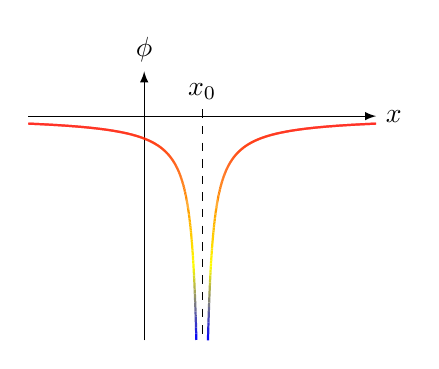
\begin{tikzpicture}
  \begin{axis}[
    width=6cm,
    height=5cm,
    colormap/hot,
    point meta max=0,
    point meta min=-10,
    point meta=y,
    xmin=-2, xmax=4,
    ymin=-10, ymax=2,
    axis x line=middle,
    axis y line=middle,
    xlabel={$x$},
    ylabel={$\phi$},
    xlabel style={right},
    ylabel style={above},
    xtick={\empty},
    ytick={\empty},
    declare function = { f(\x,\y,\xo,\yo) = -1/sqrt((\x-\xo)^2 + (\y-\yo)^2); },
    samples=1000,
    clip=false,
    ]
    \addplot[mesh,thick,domain=-2:0.9] { f(x,0,1,0) };
    \addplot[mesh,thick,domain=1.1:4] { f(x,0,1,0) };
    \draw[dashed] (axis cs: 1,0.3) node[above] {$x_0$} -- (axis cs: 1,-10);
  \end{axis}
\end{tikzpicture}
\end{document}
